\documentclass[11pt,a4paper]{report}
\usepackage{titlesec}
\usepackage{listings}
\usepackage{graphicx}
\usepackage{wrapfig}
\usepackage[hidelinks]{hyperref}
\usepackage{tikz}
\usetikzlibrary{calc}
\usepackage[utf8]{inputenc}
\usepackage[top=0.5in,bottom=0.5in,left=3.2cm,right=2.6cm]{geometry}
\usepackage{calc}
\usepackage{eso-pic}
\usepackage{placeins}
\usepackage[document]{ragged2e}
\usepackage{titling}
\usepackage{float}

\begin{document}
    
\renewcommand\bibname{References}

\titleformat{\chapter}{\bfseries\huge\centering}{}{0pt}{}{\huge}
\titlespacing*{\chapter}{0pt}{-60pt}{40pt}
\setlength{\parindent}{2em}
\setlength{\parskip}{1em}

\newenvironment{myindentpar}[1]%
  {\begin{list}{}%
          {\setlength{\leftmargin}{#1}}%
          \item[]%
  }
  {\end{list}}

\title{Android Application Implementing List View}

\author{Kashish Srivastava (185014)\\
        \and 
        Dipesh Kumar (185015)\\
        \and
        Akash Rana (185034)
}

\date{July 2020}



\pagestyle{plain}

\begin{titlepage}
    \begin{center}

        \Huge{\textbf{Android Application Implementing List View}}
 
        \vspace{0.5cm}
        
        \normalsize
       
        \vspace{10pt}
        
    	Data Structures\\
        CSD-223

        
        
        \vspace{15pt}
        
\includegraphics[height=5cm]{logo.png}
        
        \vspace{10pt}
        \textit{Submitted by:}

            Kashish Srivastava (185014)\\
            Dipesh Kumar (185015)\\
            Akash Rana (185034)
        \vspace{5pt}
        
        \begin{tabular}{c c}
            
        \end{tabular}
 
        \vspace{5pt}
        CSE (4 Year) : 
        4\textsuperscript{th} Semester
 
        \vspace{15pt}
 
        Under the guidance of
        
        \vspace{5pt}
        
        \textbf{Dr. Nitin Gupta }\\
        Assistant Professor, CSE Department\\
        National Institute of Technology, Hamirpur\\
 
        \vspace{25pt}
        
        \large
 
        Department of Computer Science and  Engineering\\
        National Institute of Technology, Hamirpur\\
      
    \end{center}
\end{titlepage}

		\section*{\Large{The Abstract}}
		
		Our goal was to develop a android application using list and file structure implementation as per instructions. This Android application is basically coded in Kotlin. This Android application will provide our student and other people with the brief information of each and every department (i.e about different branches of engineering that are available in our institute) to have the better idea of every department of our institute and its courses available in that respective department. By developing this Android application, our basic idea was to provide the clear idea of how linked list, queue, stack and sets can be used to develop a well working an application.
		\vskip 25cm
		\section*{\Large{Contents}}
	\centering
	\scalebox{1}{
		\begin{tabular} { | p {2cm} | p {8cm} | p {2cm} | }
			\hline
			\multicolumn{3} { | c | }{INDEX}\\
			\hline
			S.No. &\centering Contents & Page No. \\
			\hline
			1. & Introduction & 4 \\ [10pt]
			2. & Requirement and installation  & 5 \\ [10pt]
			3. & Android development & 6-9 \\ [10pt]
			4. & Conclusion & 10 \\ [10 pt]
			5. & References & 11 \\ [10pt]
			\hline
		\end{tabular}}
		\vfill
		\pagebreak
		\section*{\Large{Introduction}}
	
		The era of mobile technology opens the window to the android app development. The websites are vanishing and the mobile phones are emerging. It`s high time to changeform conventional form websites to apps, which has become the part of our daily routine. We are here introducing self made android application which would be a miniature part of our college website. It not only works as a website but also as a small college management software. This android application will provide our student and other managing staffs with the proper information of each and every department and of about its courses and placement. This android application is also a mobile version of the part of our institute official website.
		This android application also uses different data structures in the development of the same. The data structures used in its development are linked list, queue, arrays, hash table etc. These all the data structure are pre provided by the android development for the development of such application.\\List view is used in this application to groups several items and display them in vertical scrollable list which is a list of department of our institute and similarly linked list is used in this application to link last element with the recent one and also it allocates memory dynamically and hence these data structures are used in our application.
		\\
		This project is basically designed to provide the better idea of how data structures i.e linked list,list view,hash table and arrays can be used to develop real life android application for the betterment of the coming youth.
		\vskip 30cm
		  \section*{\Large{Requirements and Installation}}
		  
		The software and programming languages that are required to build an android application and we should also have prior knowledge about the following:-
		
		\subsection*{\Large{Kotlin}}
		
		Kotlin is a statically typed programming language for Java Virtual Machine (JVM) and JavaScript. Described as a general-purpose language, Kotlin introduces functional features to support Java interoperability. The Kotlin project was born out of the aspiration for heightened productivity. The goal was to improve the coding experience in a way that was both practical and effective.
		
		\subsection*{\Large{Android Studio}}
		
		Android Studio is an IDE, which is essentially an interface where you can enter your code (primarily Java or Kotlin) and access all the different tools necessary for development. Android Studio allows you to access libraries and APIs from the Android software development kit(SDK`s).
		
		\subsection*{\Large{Layout Editor for UI Development}}

		The Layout Editor enables you to quickly build layouts by dragging UI elements into a visual design editor instead of writing layout XML by hand. The design editor can preview your layout on different Android devices and versions, and you can dynamically resize the layout to be sure it works well on different screen sizes.
		
		\vskip 25cm
		\section*{Project Work}
		\vskip 1cm
		The basic workflow to develop a working android application can be explained using the image given below:-
		\begin{figure}[H]
		    \centering
		    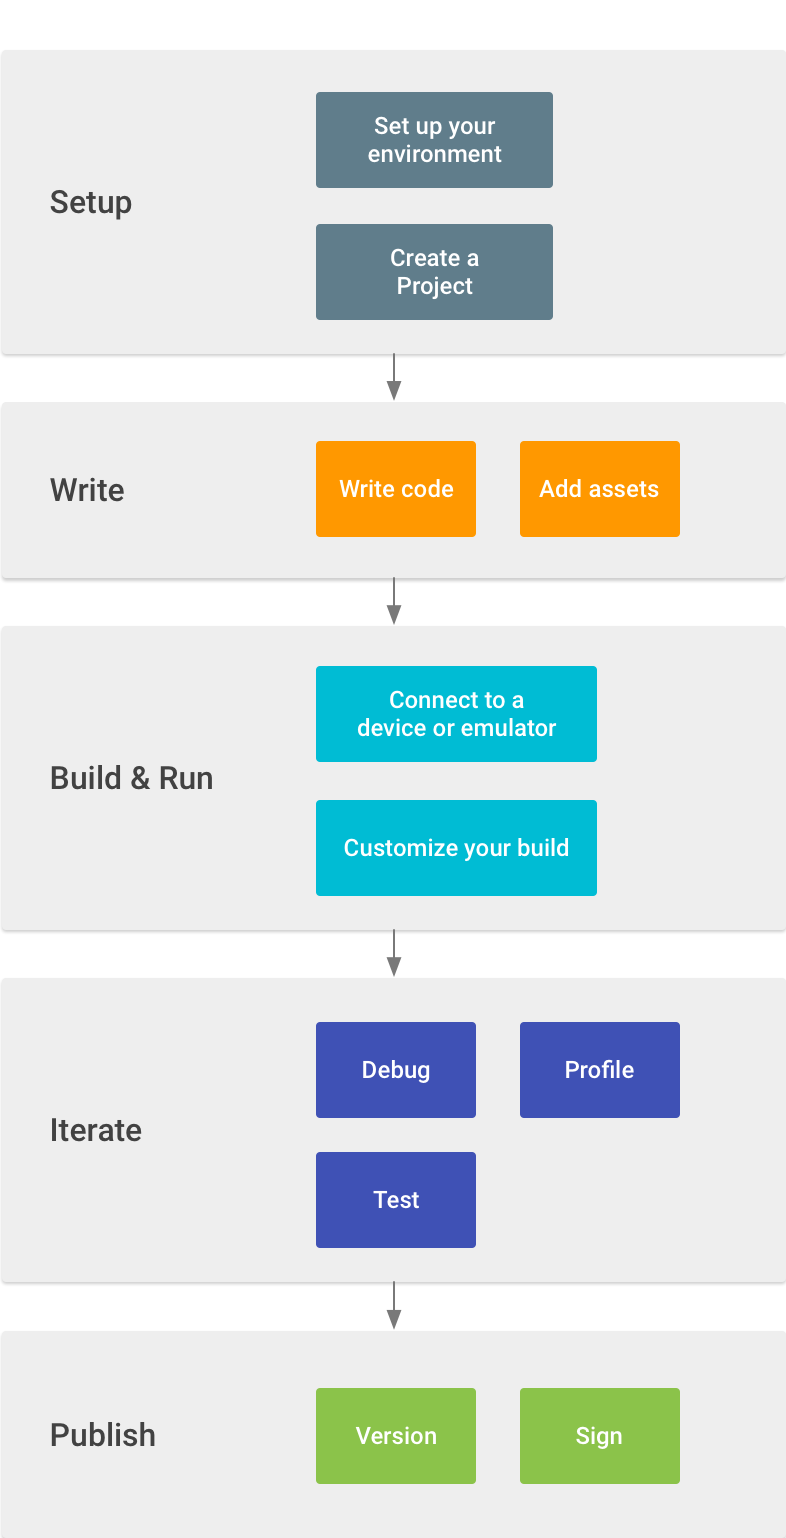
\includegraphics[scale=0.3]{developer-workflow_2x.png}
		    \caption{The workflow to develop an application with the help of data structures.}
		\end{figure}
		\vskip 7cm
		\textbf{{\large{Building an android application}}}
		\vskip 0.5cm
		To build this application we used java based language i.e kotlin to code and preferred using IDE i.e android studio.The code is written under this IDE(android studio).following are the steps that are used to create a well working android application i.e we need to create a new project in android studio and in that we created this project . in this project we used list view to display all the text in listed manner and the list view can be used in android studio using the command:-\\
		\begin{figure}[H]
		    \centering
		    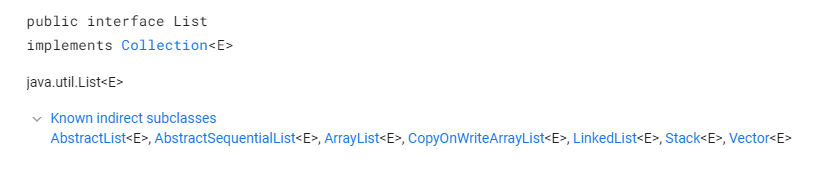
\includegraphics[scale=0.75]{Screenshot (146).png}
		\end{figure}
 	 	And in the same manner we used linked list to link the last element with the recent one as in this type of data structure recent element holds the memory address of the last element and also it allocates memory to the element dynamically and it can be used in android studio as given:-\\
 	 	   \begin{figure}[H]
 	 	       \centering
 	 	       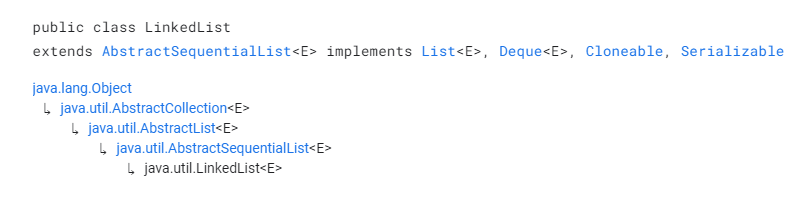
\includegraphics[scale=0.75]{Screenshot (145).png}
 	 	   \end{figure}
 	 	   After using these data structures and providing proper information according to the developing application(in our case providing information of different departments of our institute) and compiling it, we preferably counter the buges that arises in the working application so that user will not have any problem using it.
 	 	   and the final output will be like:-
 	 	   \vskip 5cm
 	 	   \begin{figure}[H]
 	 	       \centering
 	 	       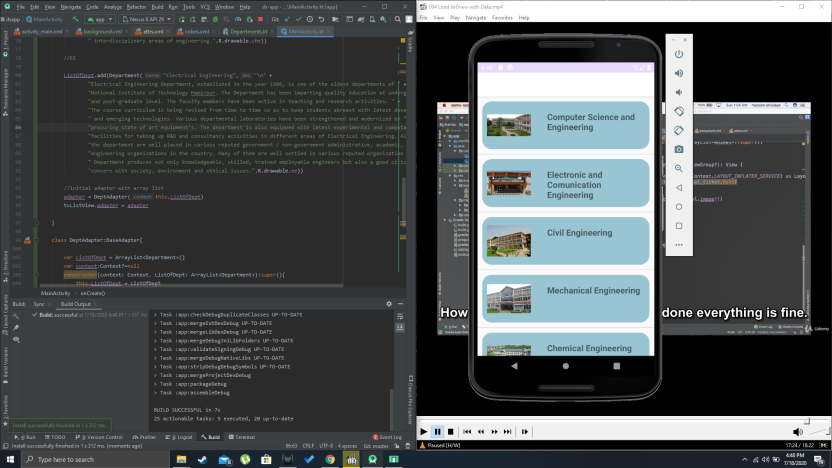
\includegraphics[scale=0.55]{Screenshot_59.png}
 	 	   \end{figure}
 	 	   \vskip 3cm
 	 	   \begin{figure}[H]
 	 	       \centering
 	 	       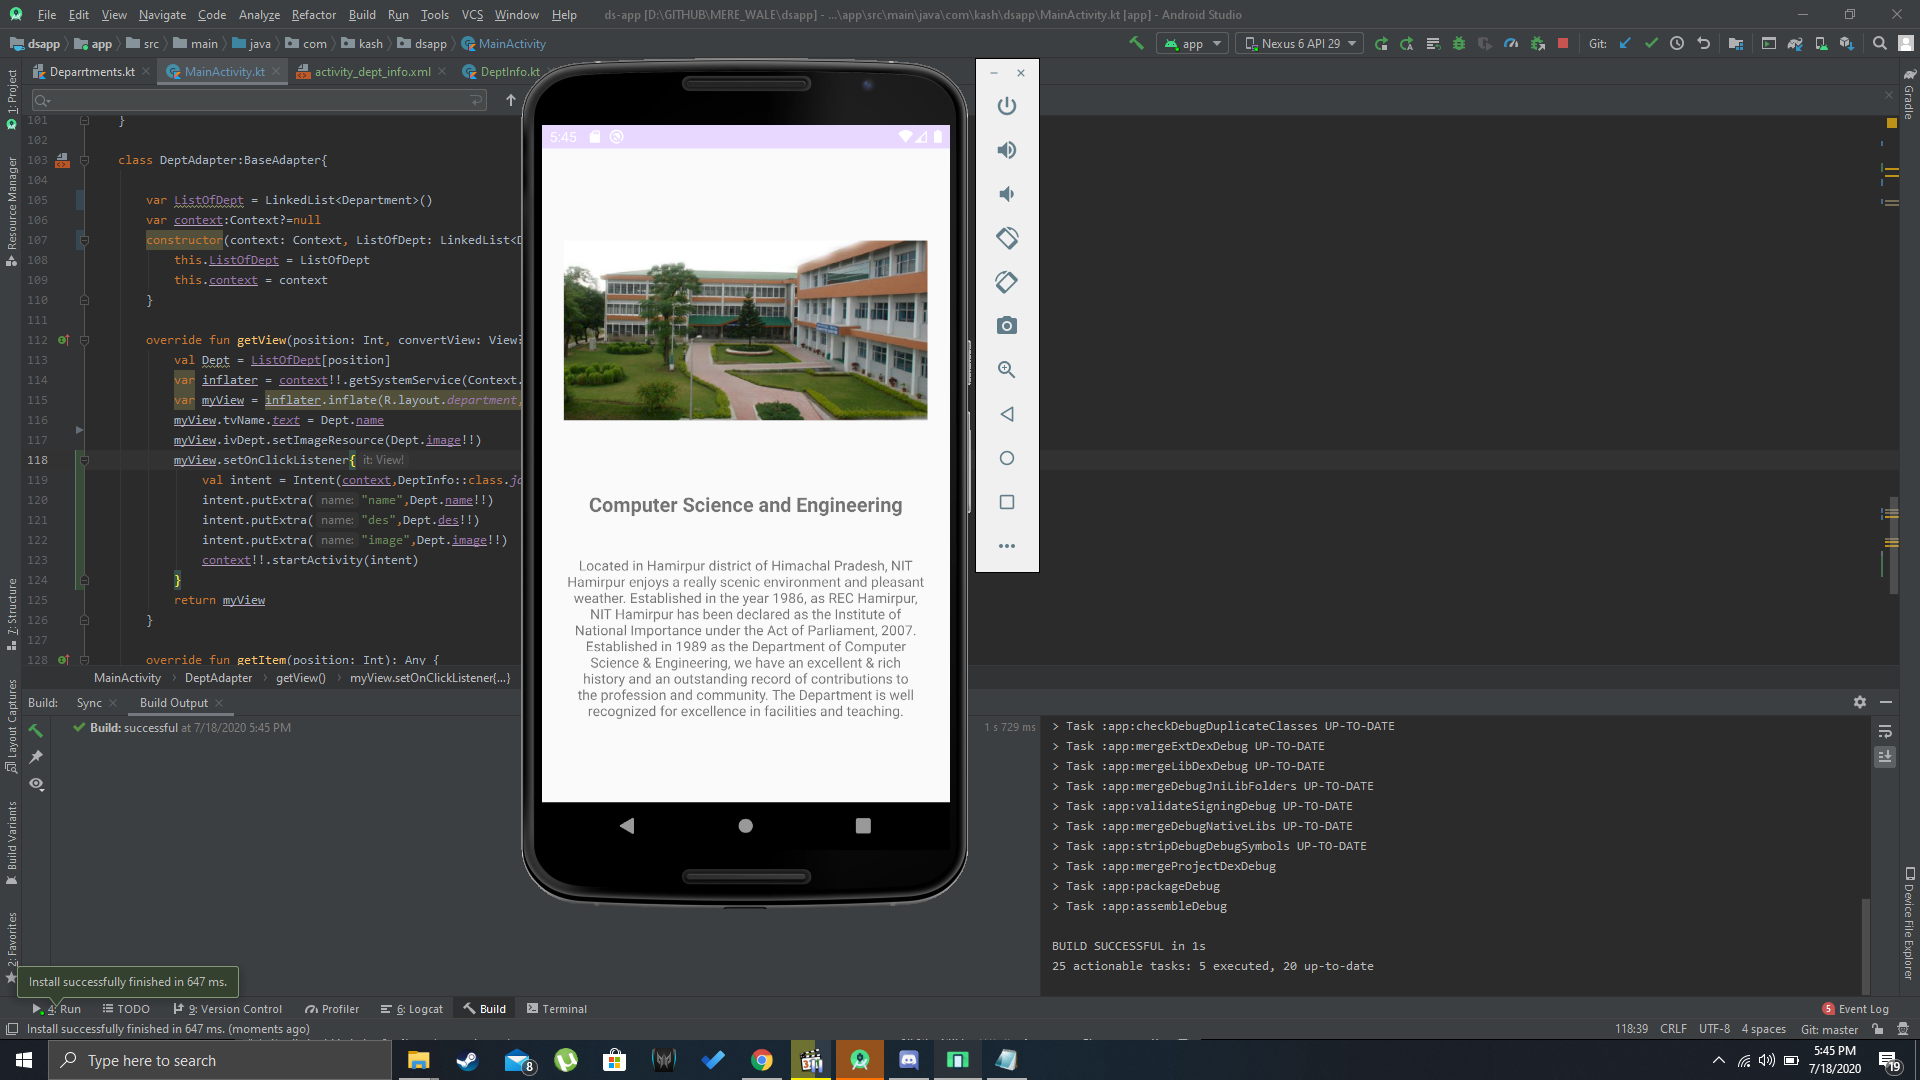
\includegraphics[scale=0.24]{Screenshot_60.png}
 	 	   \end{figure}
 	 	   \vskip 7cm
 	 	   \textbf{\large{Creating basic UI in android studio}}
 	 	   \vskip 0.5cm
 	 	   We can develop the basic user interface in android studio using layout editor.The layout controls how their child views are positioned on the screen.By using different tools and layout provided in layout editor we can make sure that how they positioned on screen and can create a beautiful user interface in android studio.\\
 	 	   \vskip 0.5cm
 	 	   And after completing all the processes and fixing all the glitches in the application,we can finally compile our project and export that project from the android studio and now this android application can be used by users to benefit themselves.
 	 	   Hence, our self developed android application (using data structure i.e list view and linked list) which is used to provide the students with the brief information of all the department of NIT Hamirpur.
		\vskip 30cm
		\section*{Conclusion}
		\vskip 1cm
		This Project was a great opportunity for us to discover new fields and ways of working.Doing this project was very interesting since our skills were really complementary. Learning kotlin and languages for this project was truly enthralling and opened new vistas for us. Indeed, it forced us to understand sound synthesis from scratch, something that always interested us. We started the project with no clear objective, and our main goal at the beginning was to build an application which will further benefit our youth in the coming future
		\vskip 0.5cm
		\begin{figure}[H]
  \centering
  \begin{minipage}[b]{0.4\textwidth}
    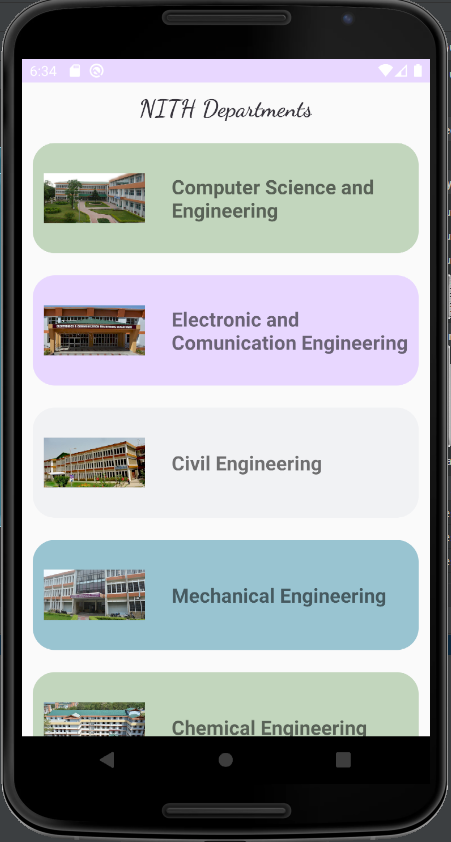
\includegraphics[width=\textwidth]{Capture1.png}
    \caption{user interface 01}
  \end{minipage}
  \hfill
  \begin{minipage}[b]{0.4\textwidth}
    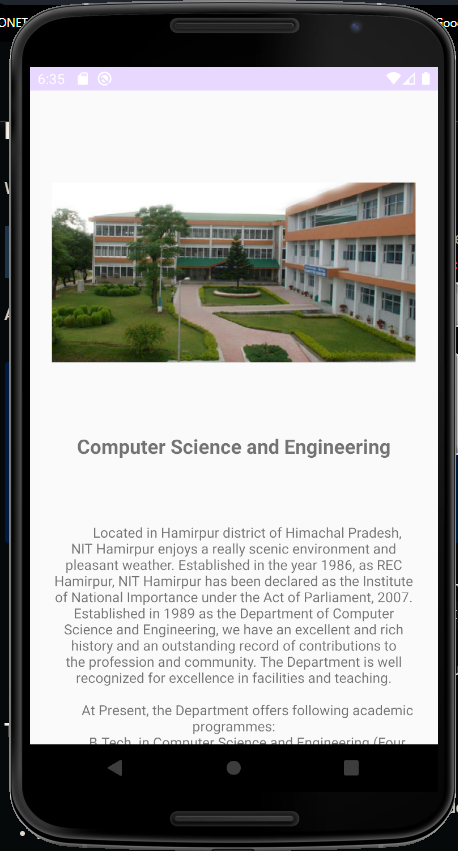
\includegraphics[width=\textwidth]{Capture2.png}
    \caption{user interface 02}
  \end{minipage}
\end{figure}

		\vskip 15cm
		\section*{References}
		\vskip 1cm
		{\large{The source code and other files related to this project can  be found at}\\
		\url{https://github.com/cannibalcheeseburger/ds-app.git}\\
		\vskip 1cm
		\large{We used following references while working with this project:-}
		\begin{itemize}
		    \item  Natarajan Raman, Eunice Adutwumwaa Obugyei, Learning Kotlin by Building Android Applications: Explore the Fundamentals of Kotlin by Building Real-world Android Applications.
		    \item Samuel Urbanowicz: Kotlin Standard Library Cookbook.
		    \item \url{https://youtu.be/PJ3RdfJ4Np8}
		    \item \url{http://developer.android.com/reference/packages.html}
		    \item \url{http://developer.android.com/guide/topics/ui/index.html}
		\end{itemize}
		}
		
		\end{document}